%% bare_conf.tex
%% V1.3
%% 2007/01/11
%% by Michael Shell
%% See:
%% http://www.michaelshell.org/
%% for current contact information.
%%
%% This is a skeleton file demonstrating the use of IEEEtran.cls
%% (requires IEEEtran.cls version 1.7 or later) with an IEEE conference paper.
%%
%% Support sites:
%% http://www.michaelshell.org/tex/ieeetran/
%% http://www.ctan.org/tex-archive/macros/latex/contrib/IEEEtran/
%% and
%% http://www.ieee.org/

% Note that the a4paper option is mainly intended so that authors in
% countries using A4 can easily print to A4 and see how their papers will
% look in print - the typesetting of the document will not typically be
% affected with changes in paper size (but the bottom and side margins will).
% Use the testflow package mentioned above to verify correct handling of
% both paper sizes by the user's LaTeX system.
%
% Also note that the "draftcls" or "draftclsnofoot", not "draft", option
% should be used if it is desired that the figures are to be displayed in
% draft mode.
%
\documentclass[conference]{IEEEtran}
\usepackage{blindtext, graphicx}
\usepackage{algorithm}
\usepackage[noend]{algpseudocode}
\usepackage[font=footnotesize,labelfont=bf]{caption}
\usepackage{placeins}
\usepackage[cmex10]{amsmath}
\usepackage{cite}
\usepackage{array}
\usepackage{mdwmath}
\usepackage{mdwtab}


% correct bad hyphenation here
\hyphenation{op-tical net-works semi-conduc-tor}


\begin{document}
%
% paper title
% can use linebreaks \\ within to get better formatting as desired
\title{Adaptive Write-Update and Write-Invalidate Cache Coherence Protocols for Producer-Consumer Sharing}


% author names and affiliations
% use a multiple column layout for up to three different
% affiliations
\author{\IEEEauthorblockN{Bangjie Liu}
\IEEEauthorblockA{Language Technologies Institute\\
School of Computer Science\\
Carnegie Mellon University\\
\texttt{bangjiel@andrew.cmu.edu}}
\and
\IEEEauthorblockN{Hao Li}
\IEEEauthorblockA{Language Technologies Institute\\
School of Computer Science\\
Carnegie Mellon University\\
\texttt{haol2@andrew.cmu.edu}}
}

% make the title area
\maketitle


\begin{abstract}
Shared memory multicore systems play crucial roles in scientific and enterprise applications. They are efficient in general applications but perform poorly in applications that establish producer-consumer sharing patterns under write-invalidate cache coherence protocol. This is because write operations trigger the invalidation of copies reside in the cache of other cores, and thus introduces a large amount of memory reads that slow the system down. This project proposes an adaptive cache coherence protocol that can eliminate unnecessary memory accesses by speculatively pushing data modified by producer to potential consumers when producer-consumer sharing patterns are detected. We evaluate the proposed adaptive protocol on ... (results)
\end{abstract}


\section{Introduction}
Shared memory multicore systems play increasingly important roles in both scientific world and the industry. Cache coherence protocol has great influence on performance of shared memory multicore systems. Producer-consumer sharing refers to situations in multi-process synchronization wherein multiple processes share a common, fixed-size buffer and some processes, as known as producers, keep writing new data to that shared buffer while some readers keep reading data from it \cite{wiki}. The most popular cache coherence protocol used in modern multiprocessor architecture is directory-based write-invalidate protocol, which is inefficient for producer-consumer sharing due to extensive invalidation traffics and expensive remote misses. This project focuses on evaluating the performance of producer-consumer application under write-invalidate and write-update protocols and proposes an adaptive protocol optimized for producer-consumer sharing patterns.

Researches have been done in this area, but they focus more on eliminating unnecessary hops by using additional hardware for cache directory and the proposed pattern detector is not sophisticated enough \cite{work1}. Instead of mitigating remote misses, this project focuses on mitigate the slowest part --- memory accesses, and proposes a sophisticated detector that investigates producer-consumer sharing patterns at a fine-grained level. More specifically, this project works on single-producer-multiple-consumer patterns and assumes that communications among caches on different cores are physically feasible.

The remainder of this report is organized as follows. We start in Section 2 with an overview of our goals and what we have accomplished. Section 3 and 4 describe the simulator in our study and our analysis of the performance of write-invalidate and write-update protocols on a representative producer-consumer application. In Section 5, we present our adaptive protocol, followed by a thorough evaluation on several applications in Section 6. Finally, we summarize our works and discuss future directions in Section 7 and 8.


\section{Goals}

\textbf{[75\%]} Implement cache simulators and testing tools (stack trace, logger, etc.) to fully evaluate and analyze the performance of directory-based write-invalidate and write-update protocols on representative multi-threaded producer-consumer applications.

\textbf{[100\%]} Implement proposed adaptive cache coherence protocols and producer-consumer sharing pattern detector. Evaluate and analyze the its performance on representative producer-consumer, as well as general-purpose applications.

\textbf{[125\%]} Equip the cache simulator with functionalities that can synchronize application threads so as to observe more accurate cache access events (mitigate the effect of pintool instrumentation).

As we write this report, we have accomplished both 75\% and 100\% goals. And due to time limits, we decide to work on a more thorough analysis of the proposed protocol on multiple benchmarks instead of the 125\% goal.


\section{Cache Simulator}
We implement a cache simulator and coherence protocols including write-invalidate, write-update, as well as the proposed adaptive versions of directory-based MSI (modified-shared-invalid) from scratch. The number of processors, cache sizes, number of sets, associativity, and line size are configurable. And it currently only simulates L1 data cache and assumes directory banks are sufficient to hold all line records. In addition, it offers load/store hit rate statistics of the entire program, each core, and even all memory accessed. Besides, it supports cycle-accurate statistics by the cost estimation in Table \ref{cost_estimation}.

% \begin{table}[!h]
% \renewcommand{\arraystretch}{1}
% \caption{Cycle Cost Estimation}
% \label{cost_estimation}
% \centering
% \begin{tabular}{|c|c|c|c|}
% \hline
% LOCAL CACHE ACCESS & REMOTE CACHE ACCESS & CACHE TO CACHE & MEMORY ACCESS\\
% \hline
% 3 & 7 & 4 & 100\\
% \hline
% \end{tabular}
% \end{table}
% \FloatBarrier

\begin{table}[!h]
\renewcommand{\arraystretch}{1.3}
\caption{Cycle Cost Estimation}
\label{cost_estimation}
\centering
\begin{tabular}{|c|c|}
\hline
LOCAL CACHE ACCESS & 3\\
\hline
REMOTE CACHE ACCESS & 7\\
\hline
CACHE TO CACHE & 4\\
\hline
MEMORY ACCESS & 100\\
\hline
\end{tabular}
\end{table}
\FloatBarrier

\newpage


\section{Write-Invalidate and Write-Update Protocols Evaluation}
In this section, we evaluate the performance, in terms of load/store hit rates, of write-invalidate and write-update protocols on a representative application that establishes producer-consumer sharing patterns. In the following evaluations, there are 1 producer and 2 consumers running on different cores. It is done on a Intel(R) Xeon(R) CPU E5-1660 v4 @ 3.20GHz machine with 32KB L1 data cache. And we only simulate L1 data cache.

\subsection{Representative Application}
In the application, there is a producer thread that keeps writing to a shared memory while there are multiple consumer threads reading for it as shown in Algorithm \ref{producer_thread} and \ref{consumer_thread}. A such self-defined application works well for evaluation purposes because it offers overall performance evaluation and more importantly a fine-grained investigation of shared memory behavior under different cache coherence protocols.

\begin{algorithm}
\caption{Producer Thread}
\label{producer_thread}
\begin{algorithmic}[1]
\State $data$ refers to a shared memory location
\While{True}
    \State GetLock() \Comment{get global lock}
    \State Produce($data$)
\EndWhile
\end{algorithmic}
\end{algorithm}

\begin{algorithm}
\caption{Consumer Thread}
\label{consumer_thread}
\begin{algorithmic}[1]
\State $data$ refers to a shared memory location
\While{True}
    \State GetLock() \Comment{get global lock}
    \State Consume($data$)
\EndWhile
\end{algorithmic}
\end{algorithm}


\subsection{Write-Invalidate Performance}
Write-invalidate protocol works poorly on producer-consumer sharing patterns. As Figure \ref{write_invalidate} indicates, the overall load hit rate is acceptable. But for the shared data alone as shown in Figure \ref{write_invalidate_1}, consumers' load hit rates are low due to a large amount of invalidation.

\begin{figure}[!h]
\centering
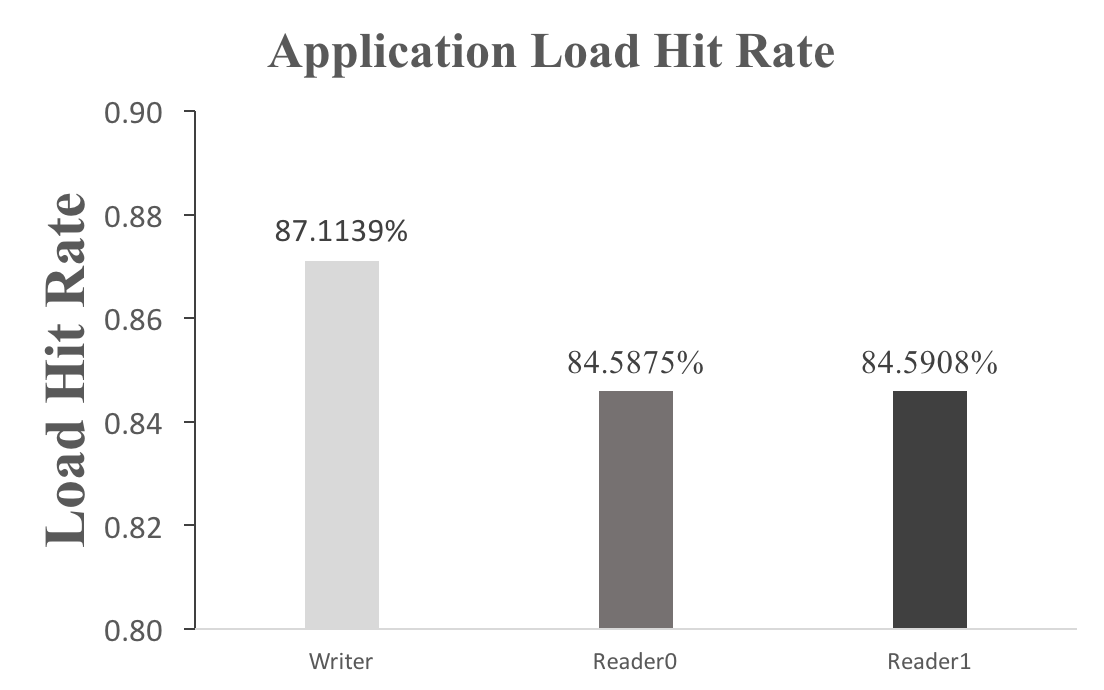
\includegraphics[width=3.5in]{write_invalidate.png}
\caption{Write-Invalidate Overall Load Hit Rates}
\label{write_invalidate}
\end{figure}
\FloatBarrier

\begin{figure}[!h]
\centering
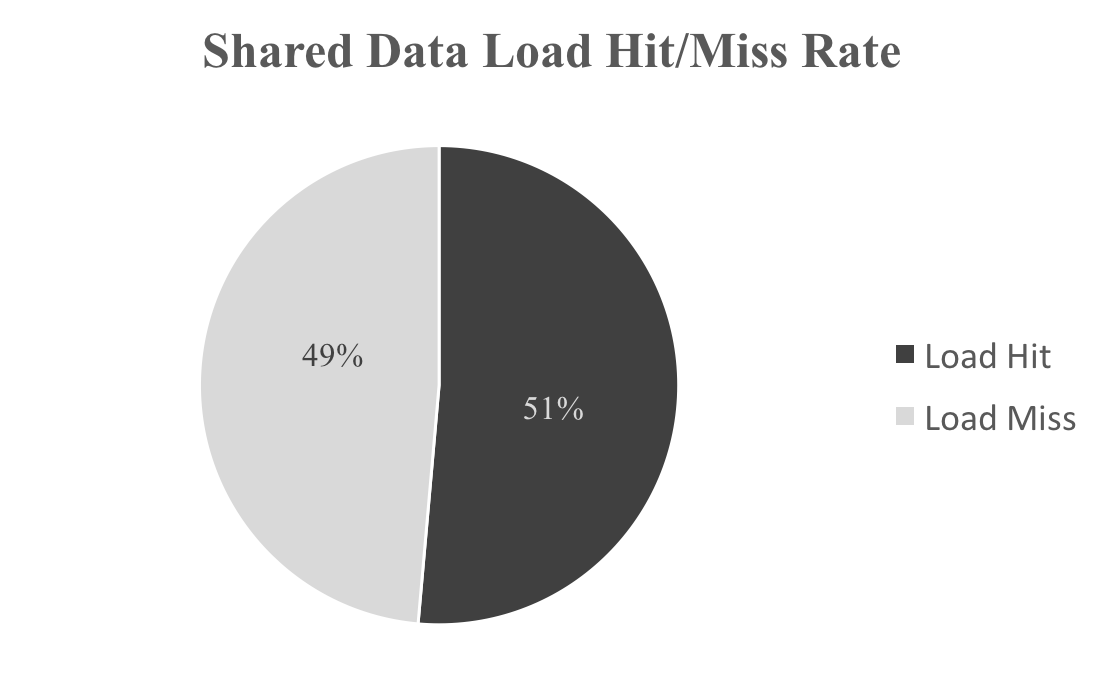
\includegraphics[width=3.5in]{write_invalidate_1.png}
\caption{Write-Invalidate Shared Data Load Hit Rates}
\label{write_invalidate_1}
\end{figure}
\FloatBarrier


\subsection{Write-Update Performance}
Write-update works well on producer-consumer sharing patterns. As Figure \ref{write_update} and \ref{write_update_1} shows, the overall performance is good and consumers have perfect load hit rates. This is because consumers now can get data via cache-to-cache communication without accessing memory.

\begin{figure}[!h]
\centering
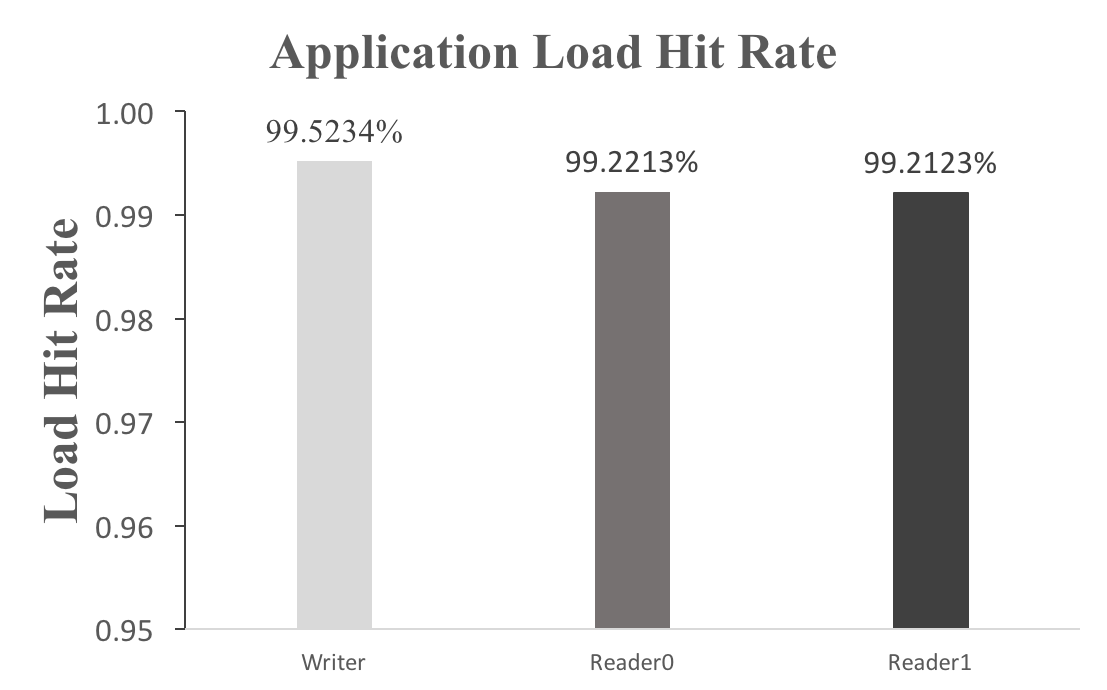
\includegraphics[width=3.5in]{write_update.png}
\caption{Write-Invalidate Performance}
\label{write_update}
\end{figure}
\FloatBarrier

\begin{figure}[!h]
\centering
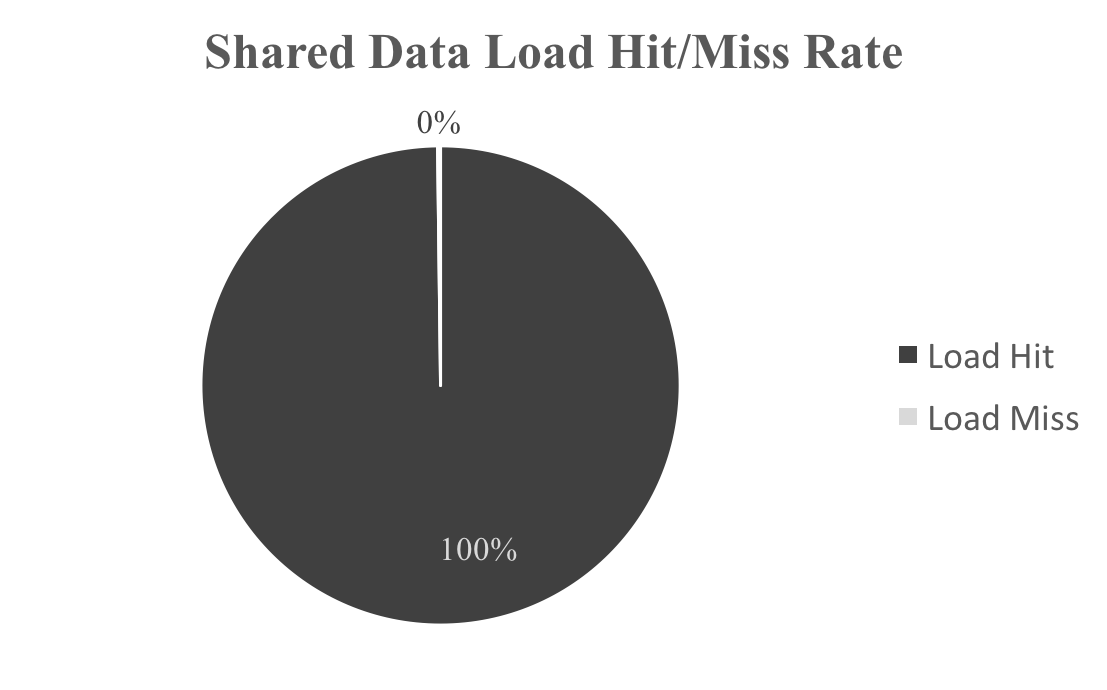
\includegraphics[width=3.5in]{write_update_1.png}
\caption{Write-Invalidate Performance}
\label{write_update_1}
\end{figure}
\FloatBarrier

\newpage

\section{Adaptive Cache Coherence Protocol}
In this section, we introduce an adaptive cache coherence protocol that intelligently switches between write-invalidate and write-update protocols. It can mitigate unnecessary memory accesses by speculatively pushing data to consumers once producer-consumer patterns are detected. Producer-consumer sharing patterns are defined as such: when a thread reads a memory location more than once after a thread writes it, the reading threads are considered as consumers of the writing thread on this particular memory location.

Additional bits are needed to track access history of each cache line for pattern identification. They are associated with directory lines which are extended to the structure shown in Figure \ref{dir_line}.

\begin{figure}[!h]
\centering
\captionsetup{justification=centering}
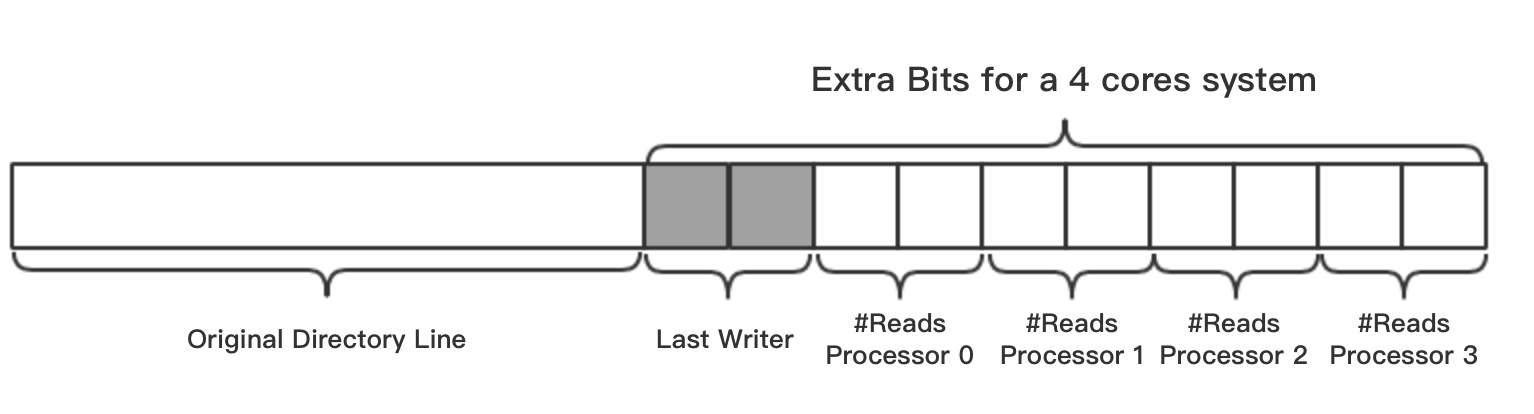
\includegraphics[width=3.5in]{dir_line.png}
\caption{Extended Directory Line Structure of a 4 Core Machine}
\label{dir_line}
\end{figure}
\FloatBarrier

The number of extra bits needed for every cache line is
\begin{equation*}
log N + 2 * N
\end{equation*}
where $N$ is the number of processors, $last\_writer$ tracks the last one to write this cache line, and there are 2 saturating bits for every processor to track the number of read operations on this cache line. Cache accesses will trigger updates on the extra bits as shown in Algorithm \ref{write_operations} and \ref{read_operations}. Note that the extra bits will be discarded to save space when its associated directory line is evicted.

\begin{algorithm}
\caption{On Write Operations}
\label{write_operations}
\begin{algorithmic}[1]
\State Let $writer\_id$ be the processor performing writes
\If{$writer\_id$ == $last\_writer$}
    \ForAll{$pid \neq writer\_id$} \Comment{exclude itself}
        \If{CountReads($pid$) $>=$ 1}
            \State Cache2CacheDataPush($pid$) \Comment{write-update}
        \Else
            \State InvalidateDataCopy($pid$) \Comment{write-invalidate}
        \EndIf
        \State SaturatingDecrease($pid$) \Comment{decrease by 1}
    \EndFor
\Else
    \ForAll{$pid \neq writer\_id$} \Comment{exclude itself}
        \State InvalidateDataCopy($pid$) \Comment{write-invalidate}
        \State ClearCount($pid$) \Comment{reset read counts}
    \EndFor
    \State UpdateLastWriter($writer\_id$)
\EndIf
\end{algorithmic}
\end{algorithm}

\begin{algorithm}
\caption{On Read Operations}
\label{read_operations}
\begin{algorithmic}[1]
\State Let $pid$ refer to a processor
\ForAll{$pid$}
    \State SaturatingIncrease($pid$) \Comment{increase by 1}
\EndFor
\end{algorithmic}
\end{algorithm}

\newpage

\section{Adaptive Protocol Evaluation}
In this section, we evaluate the performance of the proposed adaptive protocol on both general-purpose and producer-consumer sharing applications. In the following evaluations, there are 1 producer and 2 consumers running on different cores. It is done on a Intel(R) Xeon(R) CPU E5-1660 v4 @ 3.20GHz machine with 32KB L1 data cache. And we only simulate L1 data cache.

\section{Summary}

\newpage

\begin{figure}[!h]
\centering
\captionsetup{justification=centering}
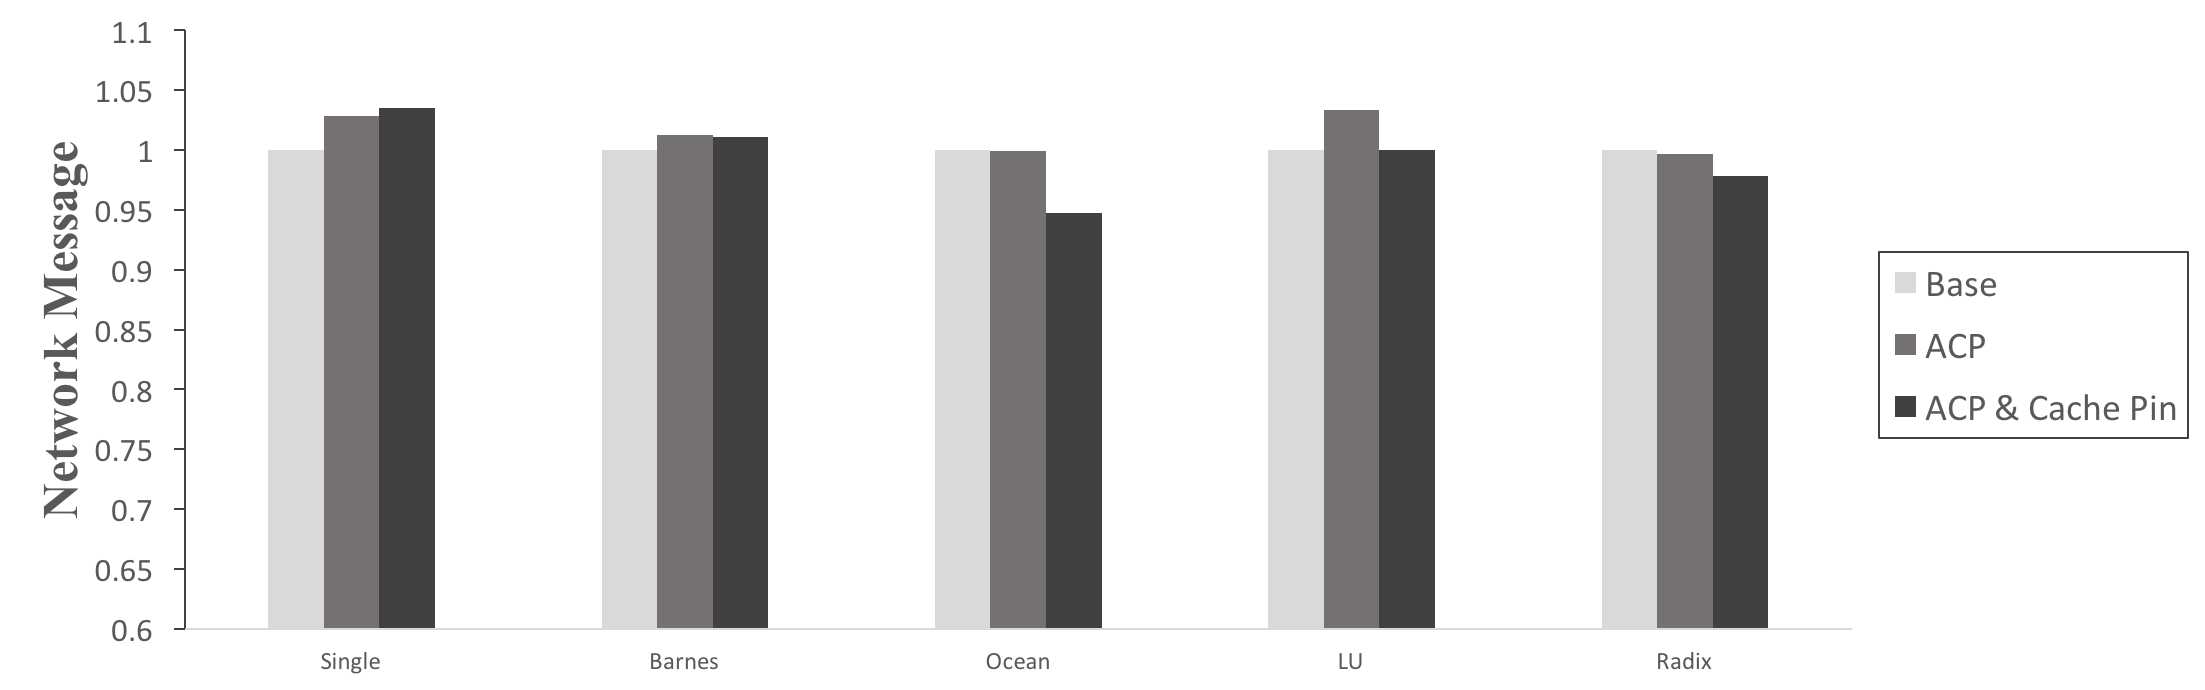
\includegraphics[width=7.35in,height=2.3in]{network_msg.png}
\caption{Network Message}
\label{network_msg}
\end{figure}
\FloatBarrier

\begin{figure}[!h]
\centering
\captionsetup{justification=centering}
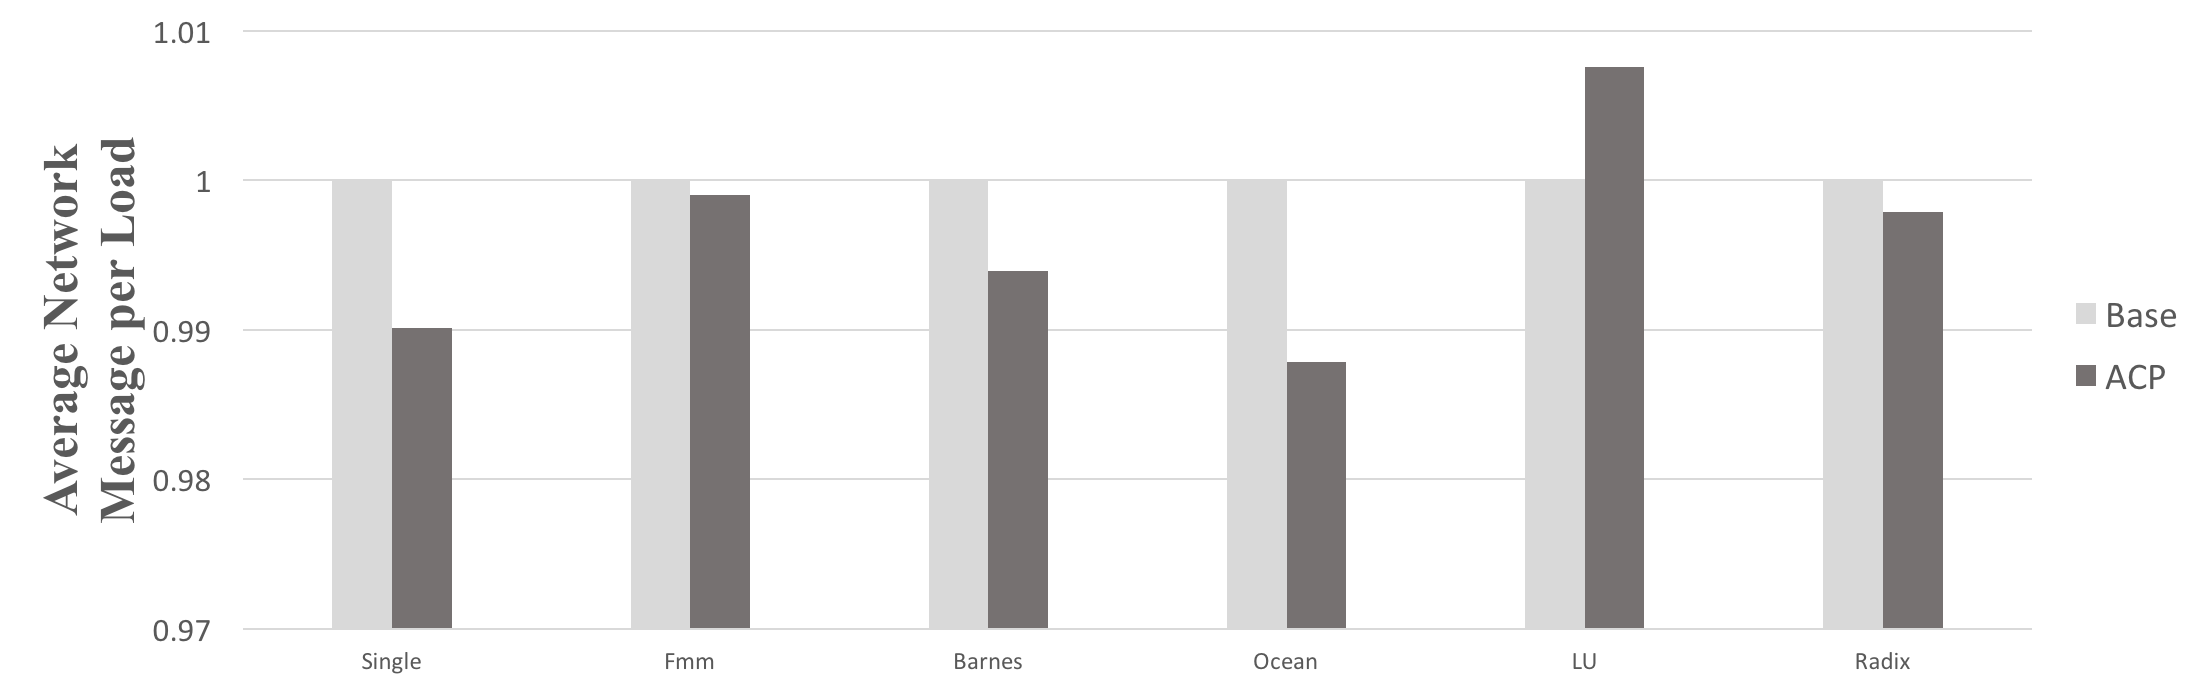
\includegraphics[width=7.35in,height=2.3in]{avg_network_msg_per_load.png}
\caption{Average Network Message per Load}
\label{avg_network_msg_per_load}
\end{figure}

\begin{figure}[!h]
\centering
\captionsetup{justification=centering}
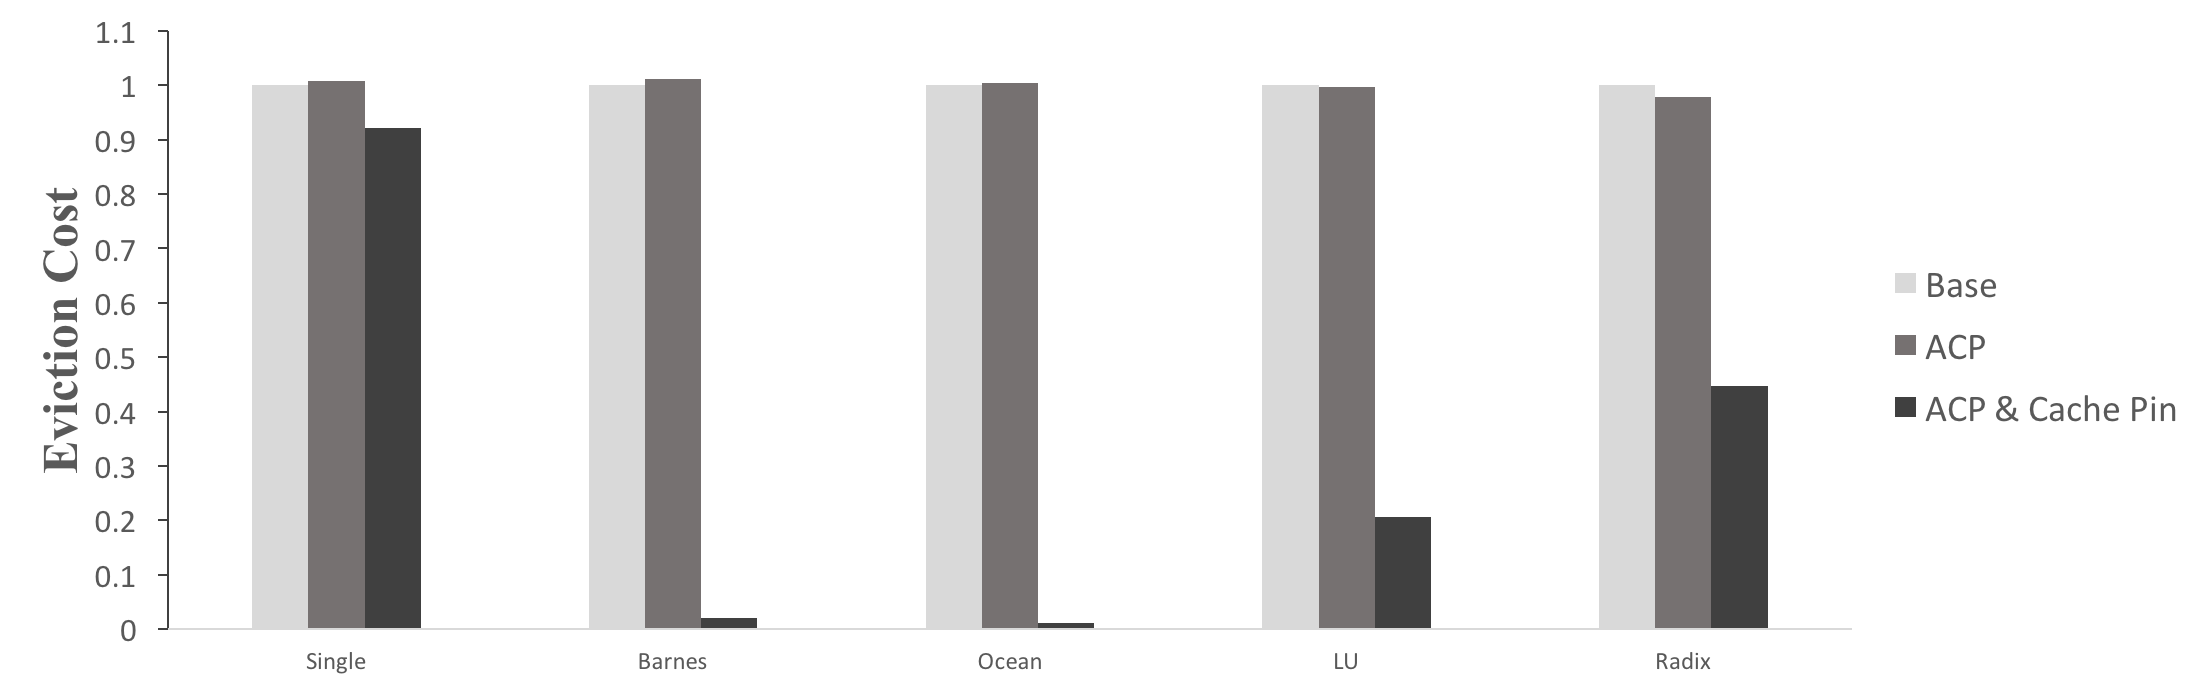
\includegraphics[width=7.35in,height=2.3in]{evict_cycles.png}
\caption{Evict Cycles}
\label{evict_cycles}
\end{figure}

\begin{figure}[!h]
\centering
\captionsetup{justification=centering}
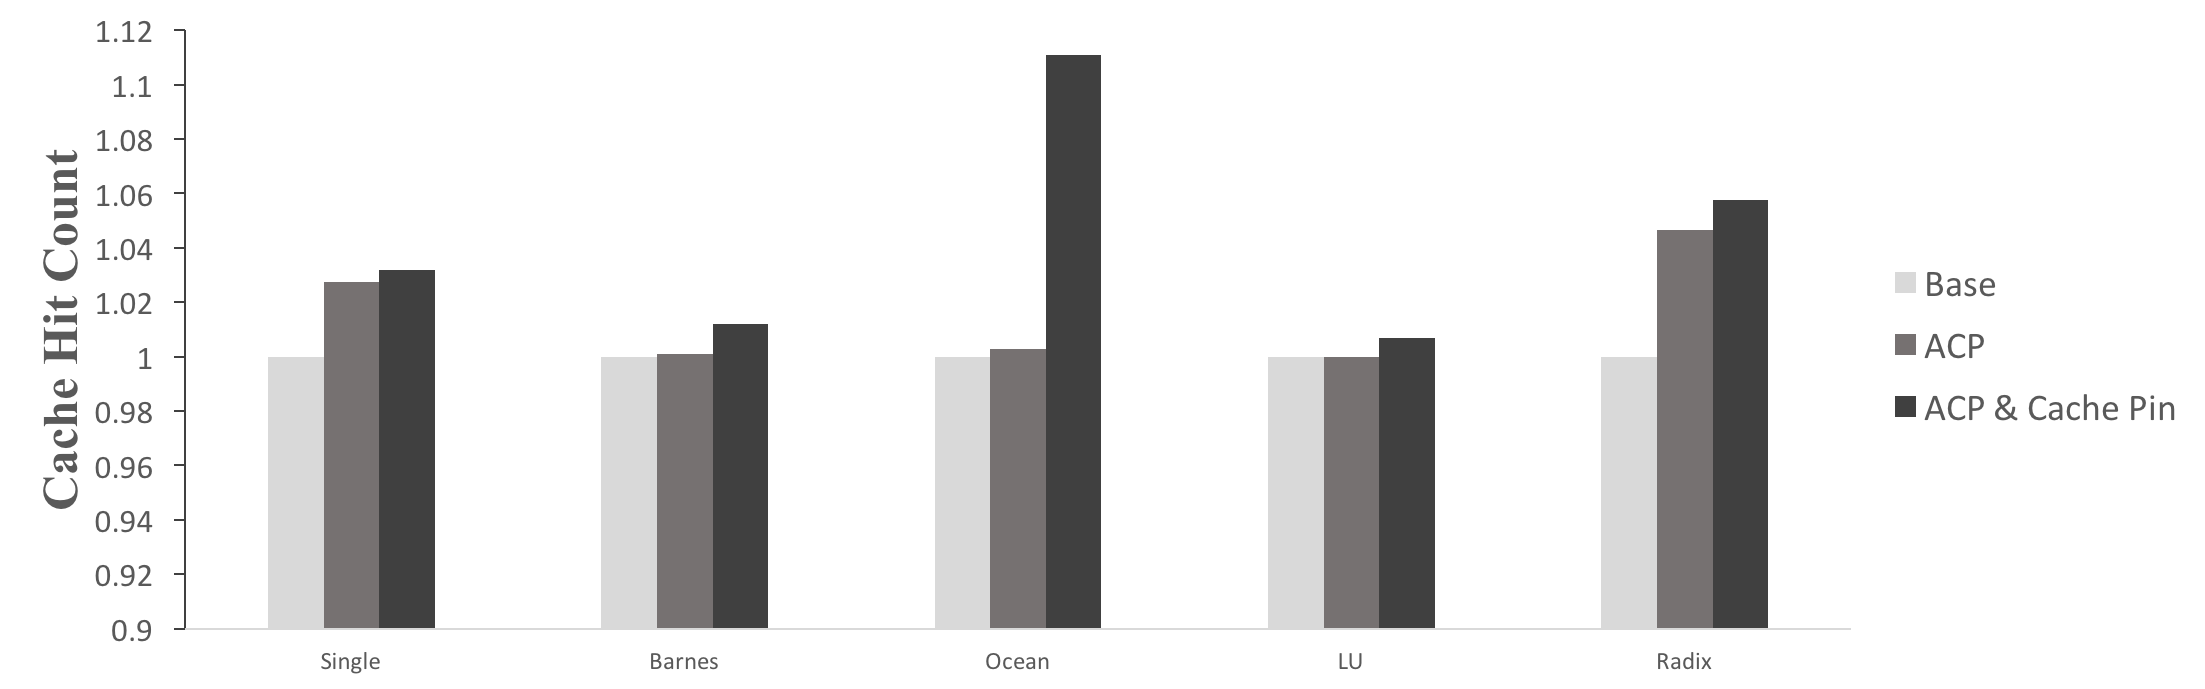
\includegraphics[width=7.35in,height=2.3in]{hit_count.png}
\caption{Hit Count}
\label{hit_count}
\end{figure}
% % \FloatBarrier

\begin{figure}[!h]
\centering
\captionsetup{justification=centering}
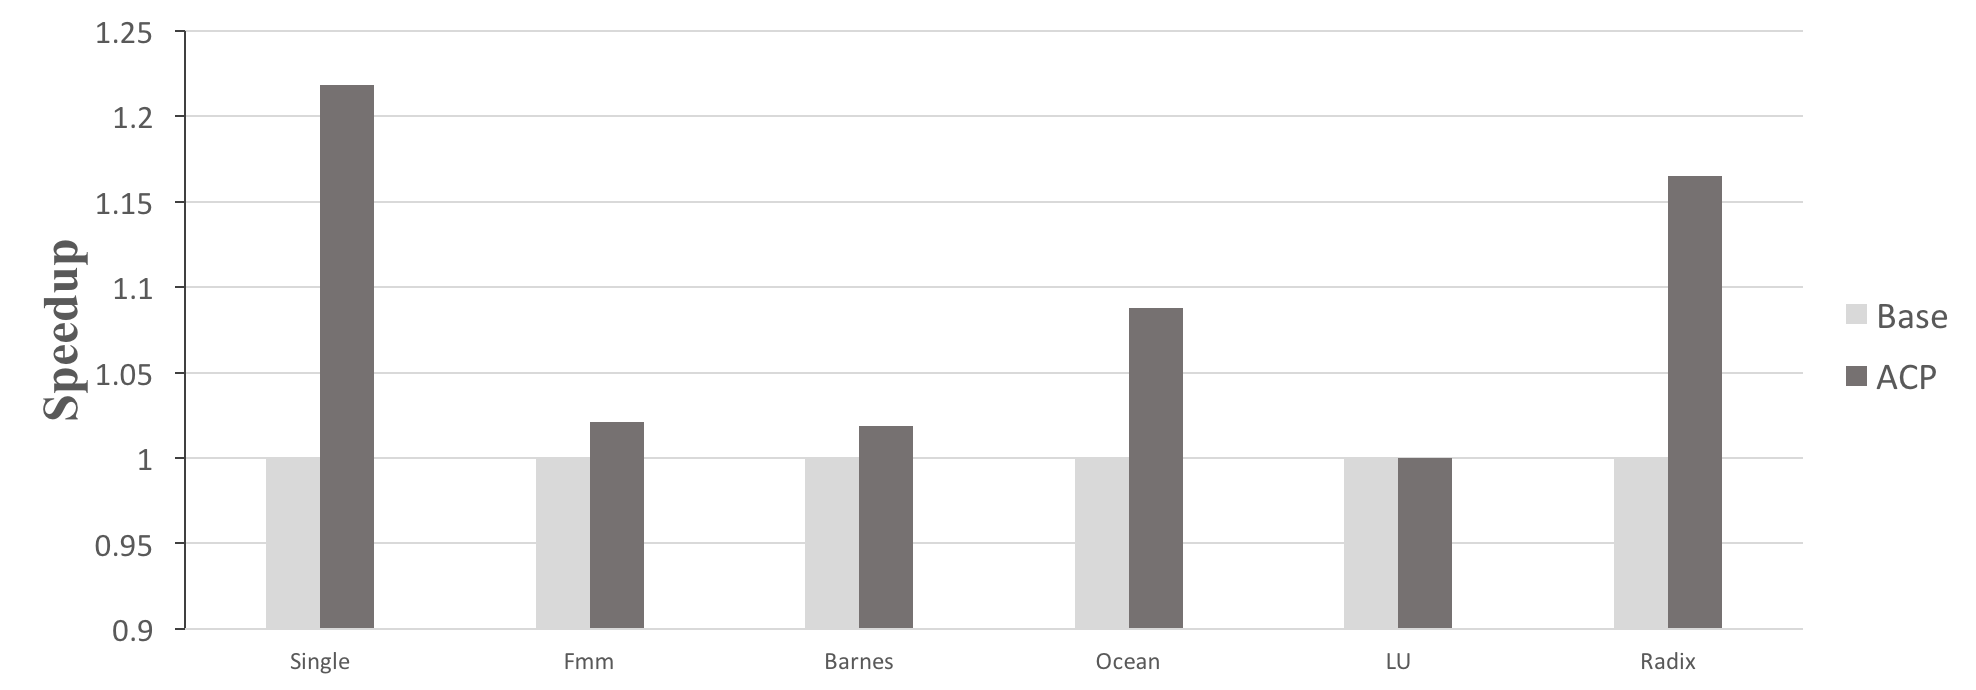
\includegraphics[width=7.35in,height=2.3in]{speedup.png}
\caption{Speedup}
\label{speedup}
\end{figure}
% % \FloatBarrier




\section{Future Works}


\newpage

\begin{thebibliography}{1}

\bibitem{wiki}
https://en.wikipedia.org/wiki/Producer-–consumer\_problem

\bibitem{work1}
Cheng, Liqun, John B. Carter, and Donglai Dai. "An adaptive cache coherence protocol optimized for producer-consumer sharing." High Performance Computer Architecture, 2007. HPCA 2007. IEEE 13th International Symposium on. IEEE, 2007.

\end{thebibliography}

\end{document}
